%%%% Semesterprojekt rapport gruppe 2 %%%%
%%%% Elektronik Q1/Q2 2016 %%%%

% Kan anvendes til journaler eller afleveringer
\documentclass[11pt, a4paper, twoside, openany]{memoir}

\usepackage[utf8]{inputenc}		% Dansk input encoding (tegn)
\usepackage[english, danish]{babel}		% Danske formuleringer / orddeling
\usepackage[T1]{fontenc}		% Output-indkodning af tegnsaet (T1)


%%% Memoir indstillinger
%% Afstand mellem afsnit og videre
%% NIX PILLE - medmindre strengt nødvendigt
\setaftersubsubsecskip{6pt}	
\setbeforesubsubsecskip{6pt}
%\setaftersubsecskip{6pt}
%\setbeforesubsecskip{-\baselineskip}
%\setaftersecskip{6pt}
%\setbeforesecskip{-\baselineskip}
%\setaftersecskip{1ex}


\raggedbottom



\chapterstyle{section}

% ¤¤ Marginer ¤¤ %
\setlrmarginsandblock{3.5cm}{2.5cm}{*}		% \setlrmarginsandblock{Indbinding}{Kant}{Ratio}
\setulmarginsandblock{3.0cm}{2.5cm}{*}		% \setulmarginsandblock{Top}{Bund}{Ratio}
\checkandfixthelayout

%%% Font valg %%%
\usepackage{mathpazo}	%Palatinofont - matematikformler
\usepackage{eulervm}		%Palatinofont

%%% FIGURER OG TABELLER %%%
\usepackage{graphicx} 						% Haandtering af eksterne billeder (JPG, PNG, PDF)

\usepackage[export]{adjustbox}

\usepackage{subfig}

\usepackage{multirow}                		% Fletning af raekker og kolonner (\multicolumn og \multirow)
\usepackage{colortbl} 						% Farver i tabeller (fx \columncolor, \rowcolor og \cellcolor)
\usepackage[dvipsnames]{xcolor}				% Definer farver med \definecolor. Se mere: http://en.wikibooks.org/wiki/LaTeX/Colors
%\usepackage{flafter}						% Soerger for at floats ikke optraeder i teksten foer deres erence
\usepackage{float}							% Muliggoer eksakt placering af floats, f.eks. \begin{figure}[H]
\usepackage{multicol}         	        	% Muliggoer tekst i spalter
%\usepackage{rotating}						% Rotation af tekst med \begin{sideways}...\end{sideways}
\usepackage{booktabs}
\usepackage{bigstrut}	% Excel2latex måskeh
\usepackage{tabularx}

%%% ¤¤ Matematik mm. %%%
\usepackage{amsmath,amssymb,stmaryrd} 		% Avancerede matematik-udvidelser
\usepackage{mathtools}						% Andre matematik- og tegnudvidelser
\usepackage{textcomp}                 		% Symbol-udvidelser (f.eks. promille-tegn med \textperthousand )
\usepackage{siunitx}						% Flot og konsistent praesentation af tal og enheder med \si{enhed} og \SI{tal}{enhed}
\sisetup{output-decimal-marker = {,}}		% Opsaetning af \SI (DE for komma som decimalseparator) 
\sisetup{exponent-product=\cdot, output-product=\cdot}	%Eksponent er gange tegn, output produkt er gange tegn
\sisetup{digitsep = none}					%Almindeligt komma - ingen mellemrum aka. til eurokomma




%%% MISC %%%
\usepackage{listings}						% Placer kildekode i dokumentet med \begin{lstlisting}...\end{lstlisting}
\definecolor{bg}{HTML}{F0F0F0}
\lstset{language=C++,
				showstringspaces = false,
				backgroundcolor = \color{bg},
                basicstyle=\ttfamily,
                keywordstyle=\color{blue}\ttfamily,
                stringstyle=\color{red}\ttfamily,
                commentstyle=\color{green}\ttfamily,
                morecomment=[l][\color{magenta}]{\#},
                extendedchars=true,
                numbers=left, numberstyle=\tiny,		% Linjenumre
                columns=flexible,						% Kolonnejustering
                breaklines, breakatwhitespace=true,		% Bryd lange linjer
                literate=%
                {æ}{{\ae}}1
                {å}{{\aa}}1
                {ø}{{\o}}1
                {Æ}{{\AE}}1
                {Å}{{\AA}}1
                {Ø}{{\O}}1
}


\usepackage{lipsum}							% Dummy text \lipsum[..]
\usepackage[shortlabels]{enumitem}			% Muliggoer enkelt konfiguration af lister
\usepackage{pdfpages}						% Goer det muligt at inkludere pdf-dokumenter med kommandoen \includepdf[pages={x-y}]{fil.pdf}	
\pdfoptionpdfminorversion=6					% Muliggoer inkludering af pdf dokumenter, af version 1.6 og hoejere

%	¤¤ Afsnitsformatering ¤¤ %
%\setlength{\parindent}{0mm}           		% Stoerrelse af indryk
\setlength{\parskip}{1.5mm}          		% Afstand mellem afsnit ved brug af double Enter
\linespread{1,1}							% Linie afstand

\usepackage{tikz}


% ¤¤ Visuelle  ¤¤ %
\usepackage[colorlinks]{hyperref}			% Danner klikbare referencer (hyperlinks) i dokumentet.
\hypersetup{colorlinks = true,				% Opsaetning af farvede hyperlinks (interne links, citeringer og URL)
	linkcolor = black,
	citecolor = black,
	urlcolor = black
}
\usepackage{url}

%%% REFERENCER %%%
%\usepackage{xr}
%\externaldocument{../dokumentation/dokumentation.tex}



%%% Referencer / Bibliografi %%%
\usepackage[backend=biber, sorting=none, style=numeric]{biblatex}
\bibliography{../referencer.bib}






\usepackage[draft, danish]{fixme}
\fxsetup{layout=footnote}

\graphicspath{{../fig/}{../fig}{fig/}{./}}

\usepackage{titlesec}

\setcounter{secnumdepth}{4}

\titleformat{\paragraph}
{\normalfont\normalsize\bfseries}{\theparagraph}{1em}{}
\titlespacing*{\paragraph}
{0pt}{3.25ex plus 1ex minus .2ex}{1.5ex plus .2ex}


%%%% Opsætning af dokument %%%%
\newcommand{\forfatter}{Gruppe 2}
\newcommand{\fag}{INDSÆT KURSUS HER}
\newcommand{\titel}{Semesterprojekt 4 Rapport}
\date{}

\author{\forfatter}
\title{\titel}


\setlength{\beforechapskip}{10pt}
\setlength{\afterchapskip}{10pt}
\begin{document}
%\maketitle
\begin{titlingpage}
%\thispagestyle{title}
\selectlanguage{danish}
		
		\begin{center}
				{\huge\bfseries Projekt Universal Actuator Drive}\\
				\vspace{10pt}
				
				{\Huge\bfseries Rapport}\\
				
				\vspace{20pt}
				
				{Diplomingeniør Elektronik}\\
				{\large Bachelorprojekt Efterår 2017}\\
				
				\vspace{10pt}
				
				Ingeniørhøjskolen Aarhus Universitet\\
				Vejleder: Arne Justesen
				\vspace{10pt}
				
				20. december 2017
				\vspace{10pt}
				\begin{figure}[H]
					\centering
					%\includegraphics[max width=0.9\linewidth]{forside.png}
				\end{figure}
				\vspace{50pt}
				\begin{minipage}{0.25\linewidth}
					\centering
					\hrule
					\vspace{12pt}
					Nicolai H. Fransen\\
					Studienr. 201404672
				\end{minipage}
				\hspace{10pt}
				\begin{minipage}{0.25\linewidth}
					\centering
					\hrule
					\vspace{12pt}
					Jesper Kloster\\
					Studienr. 
				\end{minipage}
				\hspace{10pt}


		\end{center}

\end{titlingpage}
		
		\selectlanguage{danish}
		\begin{abstract}
			
		\end{abstract}
		
		\selectlanguage{english} 
		\begin{abstract}
			
		\end{abstract}
		
		\selectlanguage{danish}
		
		\clearpage
		
	%\setcounter{tocdepth}{2}
	\tableofcontents
	\clearpage
	
	%% Synopsis:
	
	% Indholdsfortegnelse
	% Ansvarsområder
	% Abstract
	
	% Forord
	% Indledning
	% Opgaveformulering
	% Systembeskrivelse
	% Krav(specifikation)
	% Projektbeskrivelse
	%% Projektgennemførsel
	%% Udviklingsprocesser / Arbejdsmetoder
	%% (Udviklingsværktøjer); nødvendigt?
	%% Specifikation og Analyse
	%% Systembetragtning
	%% Systemarkitektur
	
	% Hardware - design og implementering
	%% Design
	%% (De forskellige moduler)
	
	% Software - design og implementering
	
	% Resultater og diskussion
	% Fremtidigt arbejde (?)
	% Konklusion
	% Ordliste (?)
	% Referencer
	
	%\include{<sti/filnavn>}
	
	
	\chapter{Indledning}
Proces er en særdeles vigtig del af et projektforløb, og består af mange forskellige elementer. En god processtruktur kan hjælpe til at give bedre overblik over perioden og gøre alle parter enige om, hvordan rapport og produkt skal udformes. Uden elementerne i en procesbeskrivelse risikerer gruppen, at arbejde i forskellige retninger, og på den måde ikke opnå optimalt samarbejde. Ved at have en række retningslinjer skrevet ned omkring, hvordan f.eks. arbejdsfordelingen og udviklingsforløbet skal foregå, er risikoen for misforståelser mindre i løbet af perioden. En veldefineret processtruktur bliver vigtigere og vigtigere, jo flere folk der arbejder sammen. Men selv i grupper af få personer, giver det optimerede arbejdsbetingelser, når der er faste måder, at gøre tingene på.  

I denne gruppe er der lagt vægt på, at opsætte en proces, der giver det bedste fundament for en god produktudvikling. Da gruppen består af to medlemmer har der med fastlagte udviklingsforløb og arbejdsfordelinger, været mere tid til udviklingen af produktet. Der er gennemgående benyttet en iterativ udviklingsproces, da det har været nødvendigt at opnå erfaring og ny viden løbende. 

Grundet gruppestørrelsen har der ikke været fordelt procesmæssige hovedansvarsområder blandt medlemmerne. Der har istedet været en flad struktur, hvor begge medlemmer har været inde over alle delene i processen.   
	
	
\chapter{Projektafgrænsning}
I dette afsnit er der beskrevet en afgrænsning af projektets indhold. Her er der taget udgangspunkt i det den ønskede funktionalitet af produktet, som sammenholdes med den egentlige opnåede funktionalitet. Elementer af projektet der er specificeret, men ikke implementeret er angivet i dette afsnit og uddybet i afsnit~\ref{future}. 

Produktets kernefunktionaliteter er prioriteret under udviklingen. Her er især prioriteret efter elementer, som kræves funktionsdygtige, før andre elementer kan udvikles. Her er udviklet en base for produktet, hvorpå flere krav og funktionaliteter skal kunne påføres.

Der blev valgt, at tage udgangspunkt i en converter med en statisk udgang. Dette ville skabe et udgangspunkt, og genere en erfaring, der ville give base for en videreudvikling til en dynamisk udgang af converteren.  

Det er valgt, at vikling af transformatoren sker af gruppen selv. Dette vil give en erfaring inden for området, der giver indsigt i hvad der er realistisk at designe efter. Derudover vil det også give et indblik i problematikkerne i vikling af en transformator. 

Converteren er designet efter de termiske krav, ved løbende vurdering og optimering af effekttabet i komponenterne.

Ved udvikling af elektroniske produkter til rumfart, kræves det udviklet med EEE-komponenter. Disse er meget omkostningsfulde, og er derfor ikke blevet brugt i projektet. Til gengælde er der brugt Terma-godkendte komponenter. Med disse komponenter har Terma en erfaring med, at opsætte disse til EEE-komponenter.  

Det blev specificeret at converteren skulle kunne operere ved et specifikt temperaturinterval. Det blev sikret ved kontrol af komponenternes specifikationer.

For at sikre en stabil indgangsspænding på converteren er det nødvendigt at implementere et indgangsfilter. Dette filter er blevet stillet tilrådighed af Terma, da det blev besluttet at fokusere andetsteds. Dette filter vil ikke blive beskrevet i denne rapport, men funktionaliteten af det er beskrevet i dokumentationen.

\fxnote{Beskriv PWM-forsyning}




	
	
\chapter{Systembeskrivelse}
Universal Actuator Drive består af to overordnede blokke. Et power-modul, der står for effektkonverteringen i converteren. Derudover et PWM-modul, der sikrer reguleringen af converterens udgang. Power-modulet består af en transformator og en MOSFET til convertering af udgangsbelastningen. Desuden et indgangs- og et udgangsfilter for filtrering af højfrekvent støj.

PWM-modulet består af to reguleringssløjfer, der regulerer udgangen efter både udgangsstrømmen og -spændingen. Denne regulering sker ved, at tilpasse duty-cyclen af det PWM-signal, der driver MOSFET'en. Disse funktionaliteter er inkluderet i PWM-controlleren. 

På figur~\ref{fig:flowdiagram} ses et flowdiagram for konceptet af Universal Actuator Drive. Det giver et overblik over hvilke scenarier, og eksterne valg, der kan påvirke flowet i systemet. Her er det især valg af udgangsbelastning, og de to reguleringssløjfer, der påvirker systemets udgang.

Systemet bliver initieret ved valg af udgangsbelastning. Det indstiller reguleringssløjferne, således at de regulerer efter den ønskede udgangsbelastning. Når belastningen aktiveres, begynder selve converterens funktionalitet. Den tilpasser switch-signalets duty-cycle efter både udgangsstrøm og -spænding, således den ønskede belastning holdes. Det forstætter indtil systemet deaktiveres, og indgangsspændingen til converteren fjernes. 

\begin{figure}[H]
	\centering
	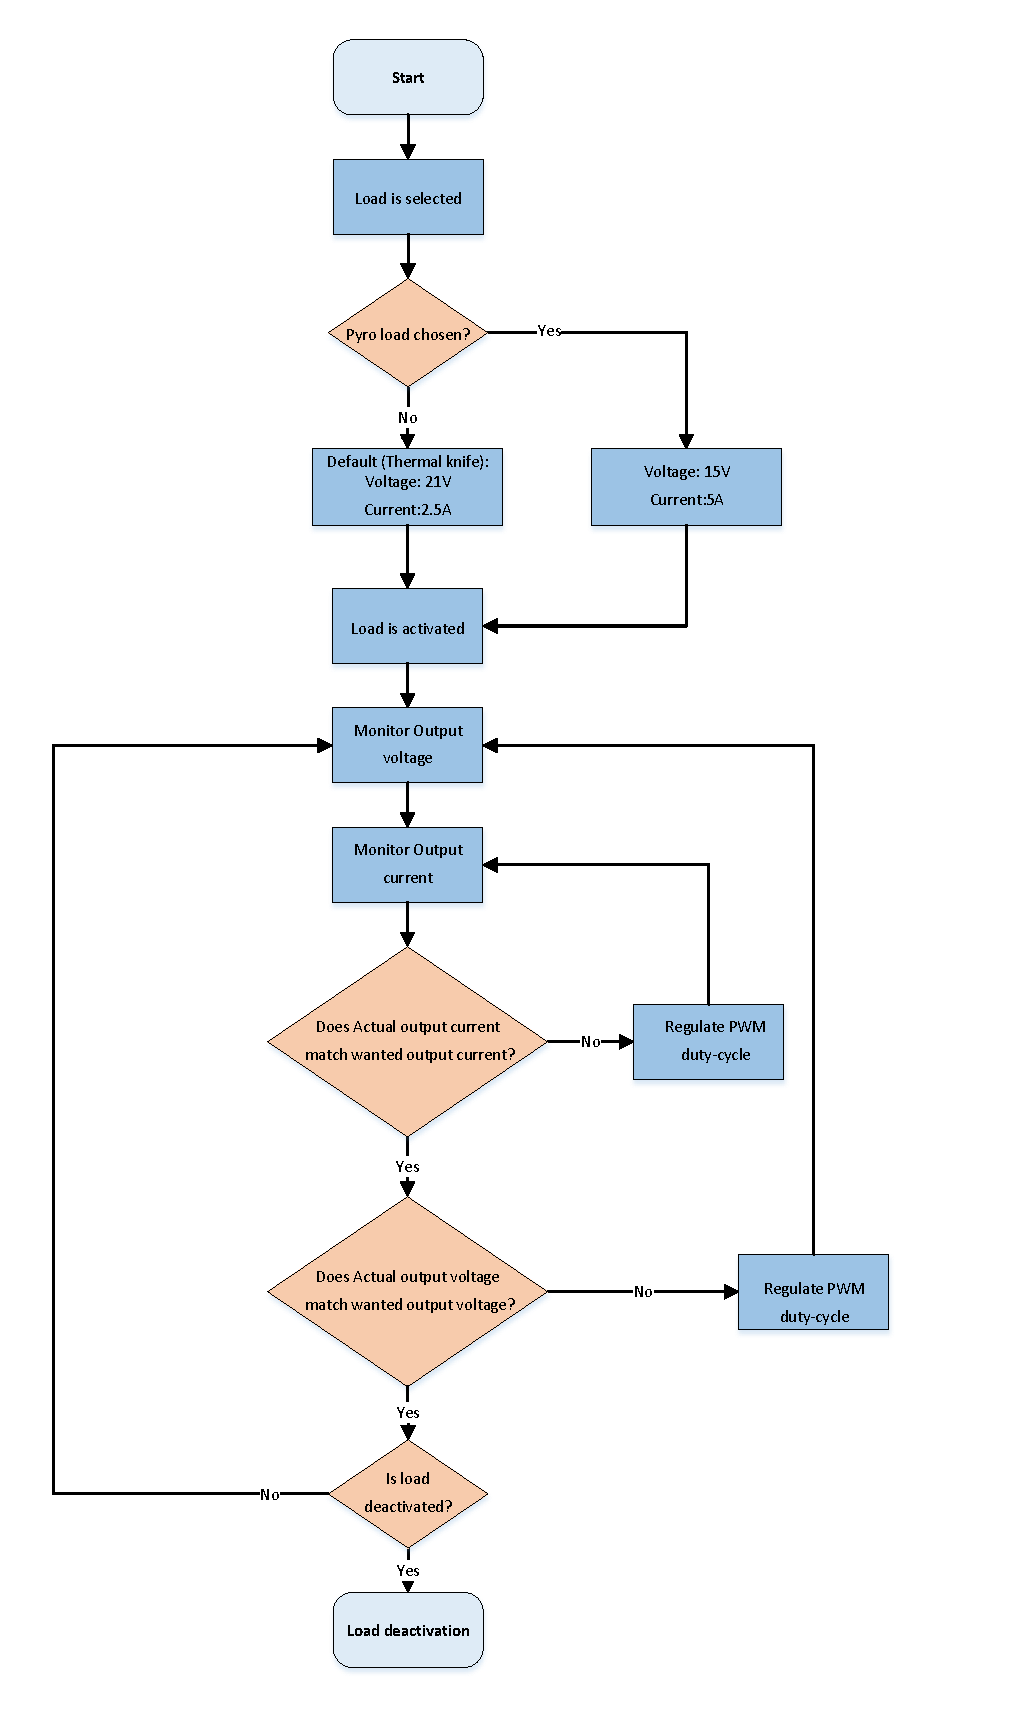
\includegraphics[width=0.7\linewidth]{../Dokumentation/tex/kravspecifikation/billeder/Flow_diagram.pdf}
	\caption{Flowdiagram for Universal Actuator Drive}
	\label{fig:flowdiagram}
\end{figure}
	
	
\chapter{Krav}
Projektets krav er specificeret, og prioriteret, vha. MoSCoW-metoden\cite{MoSCoW}. Metoden deler kravene til produktet op i fire kategorier - Must, Should, Could og Won't. Her er der prioriteret den grundlæggende funktionalitet, ved at udvikle en funktionsdygtig converter med en stationær udgang. Med dette udgangspunkt er yderligere funktionaliteter blevet ned prioriteret, og placeret i \textit{Should} og i \textit{Could}. 

\begin{itemize}
	\item[\textbf{Must}]
	\begin{itemize}
		\item Have et funktionsdygtigt power-modul
		\item Have stabil regulering
		\item Underbygges med en P-Spice model
		
	\end{itemize}
	\item[\textbf{Should}]
	\begin{itemize}
		\item Have et termisk design, kompatibelt med vakuum
		\item Have overstrømsbeskyttelse på udgangen
		\item Have overspændingsbeskyttelse på udgangen
		\item Ikke påvirke andre moduler ved fejl
		
	\end{itemize}
	\item[\textbf{Could}] 
	\begin{itemize}
		\item Have programmerbar udgangsstrøm og -spænding
		\item Konstrueres med EEE komponenter
		
	\end{itemize}
	\item[\textbf{Won't}]
	\begin{itemize}
		\item Have mulighed for brug til mere end to forskellige typer loads
		\item Have feedback til brugeren når valgt load er aktiveret
		\item Have galvanisk adskillelse
		
	\end{itemize}
\end{itemize}

\section{Kravspecifikation}
Kravene til produktet er opstillet som ikke-funktionelle krav. Det er krav der fortæller noget om kvaliteten af converteren. Det kan være krav til indgangsspændingen, præcision af udgangen og det maksimale effekttab i converteren. Der er også stillet krav til operation ved to forskellige loads, med præcision og stabilitet ved begge load typer. I dette afsnit er de mest essentielle ikke-funktionelle krav blevet nævnt, mens resten er beskrevet i dokumentationen, afsnit 1.3. Dette afsnit indeholder ligeledes de faktiske krav produktet skal overholde.


	
	
	\printbibliography[title={Litteraturliste}]

\end{document}